I amplitudemodulasjon har man det opprinnelige signalet man vil overføre,
og en carrier wave som skal \emph{bære} signalet.

Input-signalet flyttes slik at det ikke har noen negativ komponent,
deretter multipliseres det med carrier bølgen.

Resultatet er et signal med høyere frekvens hvor amplituden gir formen
til det opprinnelige signalet.

\begin{figure}[H]
  \centering
  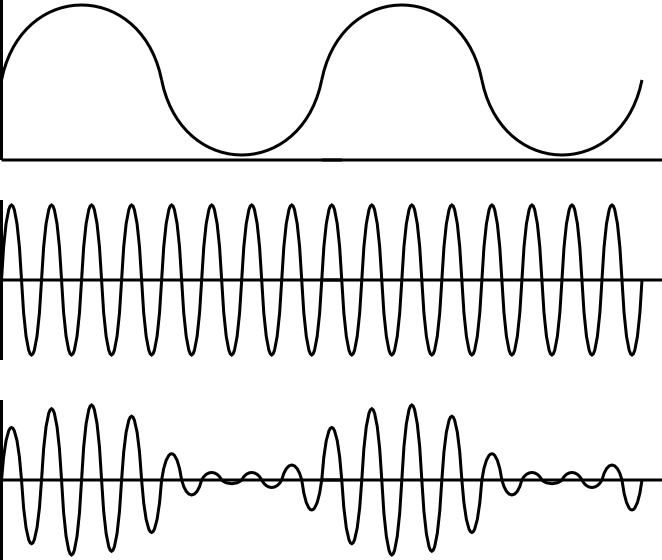
\includegraphics[width=0.67\textwidth]{./img/am}
  \caption{Input multipliseres med carrier wave}
\end{figure}
